% Narrative markers updated 3 November 2026. Target: four pages including references.
\documentclass[11pt,twoside]{article}
\usepackage{asp2023}
\usepackage{placeins}
\aspSuppressVolSlug
\resetcounters
\bibliographystyle{asp2021}
\markboth{Smallwood et al.}{Spatial Filtering in Practice}
\begin{document}
\title{Spatial Filtering in Practice: A GPU Pipeline for Real-Time RFI Mitigation}
% TODO: confirm the complete author list, affiliations, email, ADS metadata and index entries.
\author{Justin (Jay) Smallwood et al.}
\affil{Author details to be confirmed.}

\begin{abstract}
\begingroup\setlength{\emergencystretch}{1em}
We present \textit{starspin}, a new GPU-accelerated signal processing pipeline for real-time
beamforming, correlation, and radio frequency interference (RFI) subtraction
through spatial filtering on aperture arrays and phased array
feeds. The pipeline is currently being used to commission the new Low-frequency Australian Megametre-Baseline Demonstrator
Array (LAMBDA).

The theory of spatial-filtering-based RFI subtraction is well established,
building a working real-time system raises genuine systems engineering
challenges. starspin offers a flexible testbed for trialling and rapidly iterating on solutions to these challenges.
We benchmark starspin's throughput, showing
performance sufficient for processing 56.25 MHz of bandwidth on one NVIDIA RTX 4000
for the current LAMBDA array. Using LAMBDA data, we then demonstrate the pipeline's RFI subtraction on real
data.
\endgroup
\end{abstract}

\section{Motivation}

Astronomers want to make as much use of the radio spectrum as possible, but telescopes are often blinded by radio frequency interference (RFI). 
This RFI leads to contaminated data being flagged and excised. With the increase in satellites in orbit, increasing amounts of data is being contaminated and deleted. 
New methods are required to see through this RFI as an alternative to data deletion. Recent advances in graphics processing unit (GPU) performance, such as tensor cores, 
have has made software-based real-time systems viable. In this paper we will consider the application of spatial filtering to adaptively subtract RFI in real-time.


\section{Spatial Filtering}
\label{sec:beamforming}

%Radio interferometers are telescopes made up of an array of $N>1$ antennas placed at different locations.
%Each antenna senses the electric field at regular time intervals and forms a time-series of complex voltages.
%The interferometer combines these voltages into two main outputs: \textit{visibilities}, where voltages are cross-correlated with each other antenna in the array; and \textit{beams}, where antenna voltages are 
%weighted and summed to increase the sensitivity of the array to particular directions. While spatial filtering can be applied to both of these products, for brevity, we will focus on visibilities in this paper.

Spatial filtering is a mature theory with applications across many
fields, and has a long proof-of-concept history within radio astronomy.  
An interested reader is directed to the following selected papers: \cite{leshem_multichannel_2000}, \cite{kocz_radio_2010}, \cite{chippendale_interference_2017}, \cite{lourenco_mitigation_2024}, \cite{whipple_wideband_2023}.
%\cite{andrew_spatial_2026}.

%Mathematically, if $X\in \mathbb{C}^{N \times T}$, where $N$ is the number of antennas and $T$ the chosen number of integration time samples,
%the visibility matrix is formed as
%\begin{equation}
%R = XX^{*},
%\end{equation}
%where $*$ denotes the conjugate-transpose operation.
%If $w \in \mathbb{C}^{N \times B}$ is a collection of weights for $B$ beams, beams are formed by 
%\begin{equation}
%Y = w^{*} X.
%\end{equation}

When a signal arrives at an interferometer, it arrives at some antennas before others due to its propagation direction.
This characteristic pattern is called a \textit{spatial signature}.
\textit{Spatial filtering} combines the voltages from each antenna to find and augment or diminish the telescope's sensitivity to signals arriving from particular directions.
Directions of diminished sensitivity are referred to as \textit{nulls}.

%The generally accepted signal model is that under conditions of linearity of the signal chain, we get the following model of the visibilities:
%\begin{equation}
%	R = R_{v} + \sum_{i=1}^{k} \sigma^{2}_{k} a_{k} a_{k}^{*} + \sigma^{2} I
%\end{equation}
%where $R_{v}$ is the contribution of astronomical sources to the visibilities, $\sigma^{2}_{k}$ is the power of interferer $k$, $a_{k}$ its spatial signature, and $I$ represents the identity matrix of order $N$.

Adaptive spatial filtering is generally done using eigendecompositions of the visibility matrix
\begin{equation}
R = U \Lambda U^{*}
\end{equation} 
where $U$ represents the eigenvectors and $\Lambda$ is a diagonal matrix representing the eigenvalues of $R$.
This eigendecomposition will give us information on the spatial signatures of strong interfering signals, and a projection matrix calculated to suppress these directions.

Importantly, spatial filtering needs to be done on visibilities of the right timescale to avoid smearing, where one interferer can contaminate many eigenmodes. 
To quantify this, OSKAR \citep{mort_oskar_2010} was used to simulate a
low-Earth orbit satellite on various trajectories. %A interference-to-noise ratio of \(+30\) dB was used. 
%Table~\ref{tab:oskar-smearing}
%gives the integration-duration intervals in which additional significant
%eigenmodes first appear at 137.5 MHz. 
%A bracket \((a,b]\) means that a mode
%was below the threshold at \(a\) and at or above it at \(b\). 
To avoid smearing, the visibility integration time needs to become more rapid as 
elevation or frequency increase. 
For brevity, a rule-of-thumb of 50 ms integrations
is assumed.

%\begin{table}[ht]
%\centering
%\small
%\caption{Simulated OSKAR results at 137.5 MHz. Entries give the integration
%duration over which the second and fifth modes reach twice the per-antenna
%receiver-noise eigenvalue.}
%\label{tab:oskar-smearing}
%\renewcommand{\arraystretch}{1.18}
%\setlength{\tabcolsep}{18pt}
%\begin{tabular}{@{}ccc@{}}
%\hline
%& \multicolumn{2}{c}{Integration-duration bracket (s)} \\
%\cline{2-3}
%Midpoint elevation & Second mode & Fifth mode \\
%\hline
%\(15^\circ\) & \((2.00,\,2.51]\) & \(>100\) \\
%\(30^\circ\) & \((0.502,\,0.630]\) & \((39.8,\,50.1]\) \\
%\(60^\circ\) & \((0.126,\,0.158]\) & \((10.0,\,12.6]\) \\
%\(85^\circ\) & \((0.080,\,0.100]\) & \((7.94,\,10.0]\) \\
%\hline
%\end{tabular}
%\end{table}


\section{starspin: Mitigation in the Signal Chain}

starspin is an instrument-agnostic, GPU-accelerated correlator and beamformer that is designed for spatial filtering. 
While configurable, it is designed to form and filter short-term visibility matrices on the order of milliseconds, and also using this information to update beam weights. 
Corrected visibility matrices are then integrated to form long-term visibilities that are output at whatever cadence is feasible for the instrument. 
starspin is used as the correlator and beamformer from already-channelised data.
Figure~\ref{fig:starspin-architecture} shows starspin's place in the signal chain, as well as the architecture of its internals. 
starspin is written in C++ and CUDA, and makes use of libraries from RadioBlocks such as the tensor-core correlator \citep{romein_tensor-core_2021}, ccglib \citep{oostrum_ccglib}, and an as-yet-unpublished fine channeliser. 
It also uses various libraries from NVIDIA such as cuSOLVER for eigendecomposition. Front-end packet capture from ethernet is done using libibverbs.

starspin is being used as a commissioning correlator for the Low-frequency Australian Megametre-Baseline Demonstrator Array (LAMBDA) project. 
LAMBDA is a low-frequency array operating from
50–350 MHz, with the goal of adding Very Long Baseline Interferometry (VLBI) capabilities for the Southern
Hemisphere. At the time of
submission, a prototype array of 36 antennas is operational at the Paul Wild Observatory near Narrabri,
New South Wales, Australia.


We do not claim that starspin solves all of the many challenges of carrying out real-time spatial filtering. 
It does, however, provide a flexible framework for rapid testing and iteration of solutions to these 
challenges to help the community triangulate on a method that works.

\begin{figure}[ht]
\centering
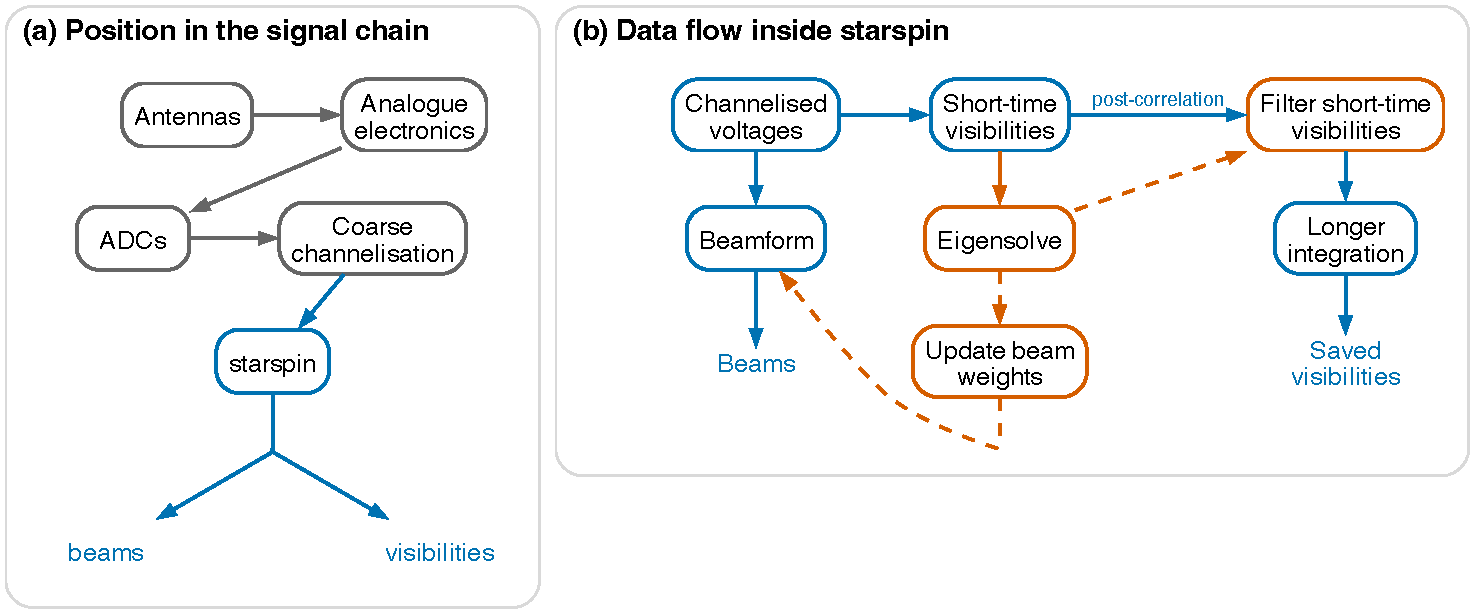
\includegraphics[width=\textwidth]{starspin_architecture.pdf}
\caption{starspin in the LAMBDA signal chain and the two filtering paths inside
the pipeline. Orange boxes represent operations relevant to filtering.}
\label{fig:starspin-architecture}
\end{figure}

\section{Benchmarks}

We present selected benchmarks from the LAMBDA production system (one NVIDIA RTX 4000 Ada, two Intel Xeon Silver 4210 CPUs). 
The server only supports PCIe 3, leading to a theoretical data transfer speed of 16 GB / s
in each direction. In practice, using pinned memory backed by hugepages, a maximum transfer speed of 
12 GB / s was reported in benchmarking tests.

We report here benchmarks from just the GPU pipeline portion of starspin, including any memory
transfers. All figures reported here use two CUDA streams, and CUDA graphs to 
reduce kernel overhead. 
Correlation and beamforming-only benchmarks both saturate the transfer limit of 
12 GB / s, corresponding to a processed bandwidth of 56.25 MHz. 
When filtering is included, this falls to 9.41 GB/s for coarse-channel filtering, and 3.72 GB/s for fine-channel filtering.
The large drop for fine-channel filtering is due to the 27-fold increase in eigendecompositions required. 
Either finding the correct balance of frequency resolution and compute capacity, or developing algorithms for more efficiently 
decomposing the visibility matrices is required.

\section{Application}

%\begin{figure}[ht]
%\centering
%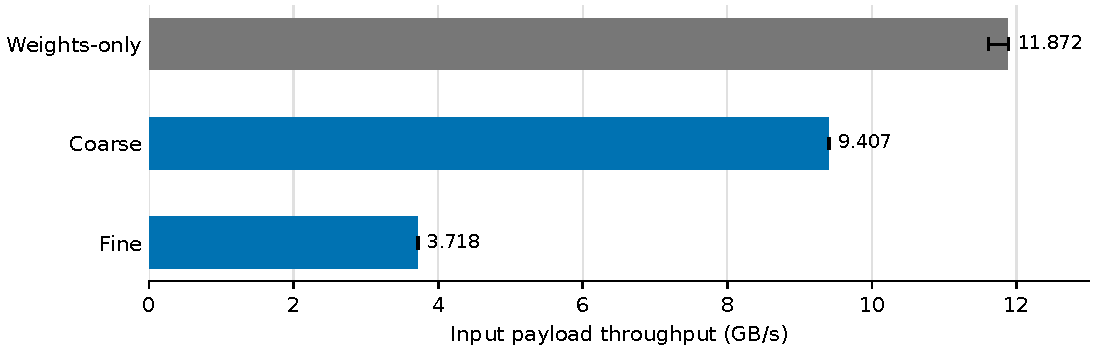
\includegraphics[width=0.96\textwidth]{starspin_two_buffer_throughput.pdf}
%\caption{Two-buffer throughput on an NVIDIA RTX
%4000 Ada. Bars show median input-data throughput. Weights-only is the
%beamforming control; Coarse and Fine each null two modes. Timing includes host-to-device
%transfer and GPU compute.}
%\label{fig:starspin-throughput}
%\end{figure}

Figure~\ref{fig:recorded-data} illustrates spatial filtering of recorded LAMBDA
data during an Orbcomm satellite pass. The goal of this experiment was to filter the data to reveal the Galactic plane, 
and compare it to the image from a nearby clean channel. As seen from panel (a), there is no Galactic plane visible in the raw dirty image; however,
the filtered image in (b) shows Galactic-plane structure similar to the clean channel in (c). Suppression of the satellite source was approximately 20 dB.

The images come from an offline analysis of \citet{smallwood_protecting_2026}, with the methodology detailed in Smallwood et al. (submitted).
However, this analysis was made possible by starspin's capture and output of visibilities at 17.7 ms. The method developed from the offline analysis
has since been added to starspin as a real-time mode.

In normal telescope operations, data from this channel would have usually been flagged and excised from analysis. 
We have shown here that it is still possible to recover useful signal from this RFI-contaminated channel.
% Assets copied unchanged from manim-animations/src/manim_animations/adass/images/
% adass_window1_{raw,protected,clean}.png, used by AliveGalacticResult in
% spatial_filtering_alive.py. These are Window 1 panels from Paper1's
% haslam_fixed2_dirty_protection_120s_sun_shrunk figure, prepared for the talk
% with only the Sun-position circles and their halos removed.
\begin{figure}[ht]
\centering
\begin{minipage}[t]{0.32\textwidth}
\centering
\small (a) Before: 137.5 MHz\par
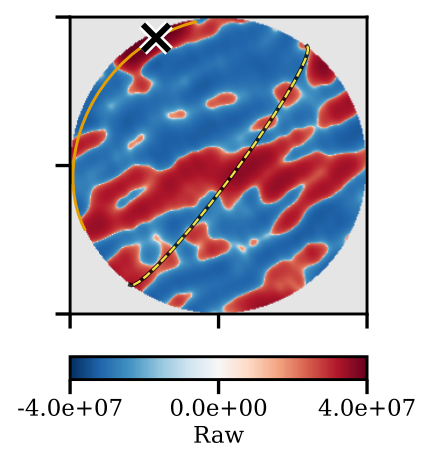
\includegraphics[width=\linewidth]{C802_f3a.png}
\end{minipage}\hfill
\begin{minipage}[t]{0.32\textwidth}
\centering
\small (b) After: 137.5 MHz\par
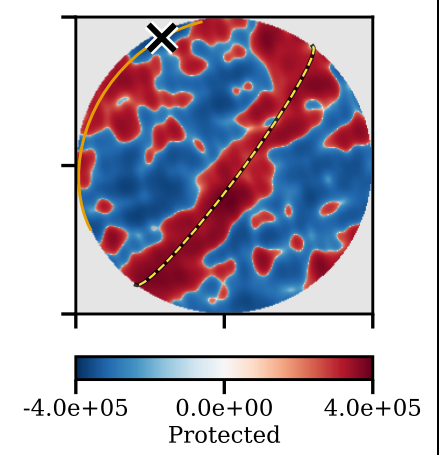
\includegraphics[width=\linewidth]{C802_f3b.png}
\end{minipage}\hfill
\begin{minipage}[t]{0.32\textwidth}
\centering
\small (c) Reference: 134.375 MHz\par
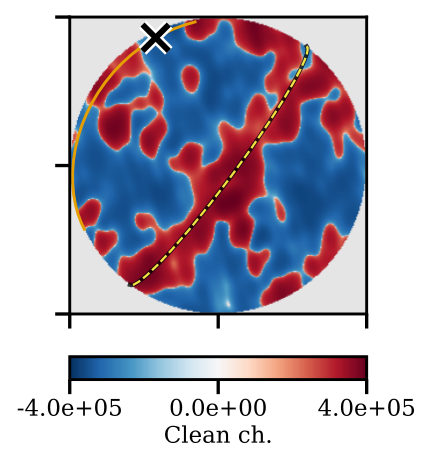
\includegraphics[width=\linewidth]{C802_f3c.png}
\end{minipage}
\caption{Dirty all-sky images from the same 120-second LAMBDA observing window:
(a) unfiltered satellite-affected data; (b) two-mode nulling; and (c) a nearby, relatively clean channel. 
The orange track and cross show the satellite ephemeris and midpoint
position; the dashed yellow line marks the Galactic plane. Filtering and imaging were performed offline.}
\label{fig:recorded-data}
\end{figure}

\section{Limitations and Further Filtering Work}
Much work remains to solve the challenges of real-time operation. 
Algorithms for calculating the number of interfering signals at each point-in-time need to be 
evaluated. Statistical properties of integrating corrected short-term visibilities such as bias must be
characterised and corrected. Information must be optimally 
combined over polarisation, time, and frequency in order to more efficiently place nulls.
A priori information about the orbit and frequency ranges of 
publically-known satellites which can also be used to more accurately place spatial nulls.



\FloatBarrier
\bibliography{C802}
% TODO: acknowledgements and subject/software index entries before submission.
% \bookpartphoto[width=1.0\textwidth]{foobar.eps}{FooBar Photo (Photo: Any Photographer)}
\end{document}
